\documentclass[a4paper,12pt]{article}
\usepackage{graphicx}
\begin{document}


\title{ EP1 de Sistemas Operacionais}
\author{ Thiago de Gouveia Nunes e Wilson Kazuo Mizutani}
\maketitle

\section{Iniciando com xv6 e QEMU}
    Primeiramente, instalamos o QEMU usando o comando aptitude install qemu-
common. Após isso, baixamos o código do xv6 e compilamos. Não foi necessário
mudar nenhum parametro no MakeFile do xv6. Depois disso, usando o comando ls
depois de usar o make qemu, obtivemos a saída que está no arquivo ls.txt.

\section{Estados de um processo xv6}

    Os estados dos processos estão com os mesmos nomes os quais são encontrados
nos arquivos do xv6. As setas indicam as mudanças de estado de um processo. O
nome perto das setas é o nome da função que modifica o estado de algum processo.
A maioria das funções muda o estado do processo proc.
\begin{center}
	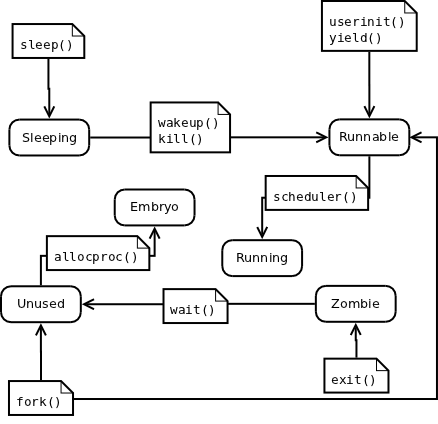
\includegraphics[scale=0.40]{state.png}
\end{center}

\end{document}
